\documentclass[a5paper,11pt]{article}
\usepackage[utf8]{inputenc}
\usepackage[left=3cm,right=2.5cm,top=3cm,bottom=2cm]{geometry}
\usepackage[dvipsnames]{xcolor}
\usepackage{graphicx}
\usepackage[rightcaption]{sidecap}
\usepackage{caption}
\usepackage{fancyhdr}
%-----------------------------------------------------------------------
\pagestyle{fancy}
\begin{document}
\pagecolor{pink}
%-----------------------------------------------------------------------
\hspace{0.5cm}{\textbf{\huge\textsf{\textcolor{cyan}{EL} 
\textcolor{red}{MEJOR} \textcolor{RubineRed}{ANIME} \textcolor{YellowOrange}{DEL}}}}

\hspace{2.5cm}{\textbf{{\huge\textsf{\textcolor{LimeGreen}{UNIVERSO}}}}}
\lfoot{Rodriguez Vega Nayeli}

\section{La mejor historia}
\subsection{Fairy Tail}
 Es una serie japonesa (anime) la cual nos cuenta que en un mundo alternativo existe la magia, la cual es utilizada comercialmente, sin embargo, el lugar en donde se desarrolla la historia es en el país de Fiore el cual contiene los principales gremios. No obstante, aquellas personas que dominan la magia se le llaman magos, los cuales son agrupados en gremios que para ser identificados de que gremio pertenecen tienen una marca que los identifica de que gremio pertenesen, la función de los gremios es que ofrecen sus servicios a cambio de dinero, es decir so contratados, para que los magos encuentren un tesoro, maten monstruos, deshagan maldiciones, etc. Uno de los gremios que se enfoca la serie es Fairy Tail el cual a lo largo de la historia nos empieza a contar principalmente las aventuras de Natsu dragneel y de sus amigos y de cómo se llegan a enfrentar a diferentes enemigos que quieren perturbar la paz de la humanidad.
 
\subsection{El mejor mago de la serie} 
\begin{enumerate}
    \item Autor: Hiro Mashima
\end{enumerate}
\subsection{La voz de la luna}
Actores de doblaje de los personajes principales:
\begin{enumerate}
    \item Natsu Dragneel: \fcolorbox{RubineRed}{Sepia}{\textcolor{RubineRed} {Tetsuya Kakihara}} y Tetsuya Kakihara (voz de niño).
    \item Lucy Heartfilia:\fcolorbox{Apricot}{brown}{\textcolor{Apricot} {Aya Hirano.}}
    \item Erza Scarlet:\fcolorbox{Turquoise}{BlueViolet}{\textcolor{Turquoise} {Sayaka Ohara.}}
    \item Gray Fullbuster: \fcolorbox{Plum}{TealBlue}{\textcolor{Plum} {Yūichi Nakamura}} y Eri Kitamura (voz de niño).
    \item Happy:\fcolorbox{GreenYellow}{OliveGreen}{\textcolor{GreenYellow} {Rie Kugimiya.}}
    \item Wendy Marvell: \fcolorbox{BrickRed}{NavyBlue}{\textcolor{BrickRed}{Satomi Satō.}} 
    \item Charlie:\fcolorbox{MidnightBlue}{Lavender}{\textcolor{MidnightBlue} {Yui Horie.}}	
\end{enumerate}
\subsection{La voz de las estrellas}
Actores de doblaje de los personajes Secundarios:
\begin{enumerate}
    \item Makarov Dreyar:Shinpachi Tsuji.
    \item Juvia Loxar:Mai Nakahara.
    \item Gajeel Redfox:Wataru Hatano.
    \item Laxus Dreyar:Katsuyuki Konishi y Hideyuki Hayami(voz de niño).
    \item Mirajane Strauss:Ryōko Ono.
    \item Cana Alberona:Hiroki Yasumoto.
    \item Mystogan:Daisuke Namikawa
    \item Levy McGarden: Levy McGarden.
\end{enumerate}
%-----------------------------------------------------------------------
\subsection{Los polvos magicos}
\begin {itemize}
    \item[$\heartsuit$]\fcolorbox{red}{yellow}{\textcolor{red} {Natsu Dragneel:}} Es un joven que utiliza la magia de fuego de dragon slayer, se marea al estar en un transporte publico,es muy divertido, muy fuerte y siempre esta acompañado de su gato llamado Happy.
    \item[$\heartsuit$]\fcolorbox{yellow}{magenta}{\textcolor{yellow} {Lucy Heartfilia:}}Es una chica alegre y una maga estelar, que a través de Llaves Estelares  puede invocar a los Espíritus Estelares.
    \item[$\heartsuit$]\fcolorbox{blue}{red}{\textcolor{blue}{Erza Scarlet:}}Es una chica que tiene el color de su cabello rojo, su magia es reequipamiento, pero ella es la única que puede re-equipar sus armas y sus armaduras. Igualmente podemos destacar que es amable, bondadosa y esla mujer mas fuerte del gremio de Fairy Tail, 
    \item[$\heartsuit$]\fcolorbox{cyan}{gray}{\textcolor{cyan}{Gray Fullbuster:}}Es un joven que tienen el cabello negro, su es de hielo y tiene la constumbre de quitarse la playara en cualquiermomento, es amable, bondadoso, aunque aveces se llega a peliar con natsu.
    \item[$\heartsuit$]\fcolorbox{orange}{green}{\textcolor{orange}{Happy:}}Es gato azul con alas que puede hablar y su magia consiste en volar, nació de un huevo y Natsu lo llamó Happy porque su llegada hizo feliz a todo el Gremio, igualmente podemos decir que es un Exceed perteneciente a Édolas.
    \item[$\heartsuit$]\fcolorbox{YellowOrange}{blue}{\textcolor{YellowOrange}{Wendy Marvell:}}Es una niña muy amable, bondadosa, inocente, fuerte que utiliza la magia de viendo de dragon slayer, igualmente se marea al estar en un transporte publico alvenos de que ocupe un echiso para controlar el mareo y simpre se encuentra acompañado de su gatita charlie.
    \item[$\heartsuit$]\fcolorbox{pink}{violet}{\textcolor{pink}{Charlie:}}Es una gatita de color blamco con alas que puede hablar y su magia consiste en volar,igualmente podemos decir que es un Exceed perteneciente a Édolas, asimismo podemos decir que es una persona muy responsable y proteje mucho a Wendy.
  \end{itemize}
%-----------------------------------------------------------------------
\subsection {El poder de las hadas}
\begin{figure}[h]
 \raggedleft
      \caption*{ Fairy tail}
      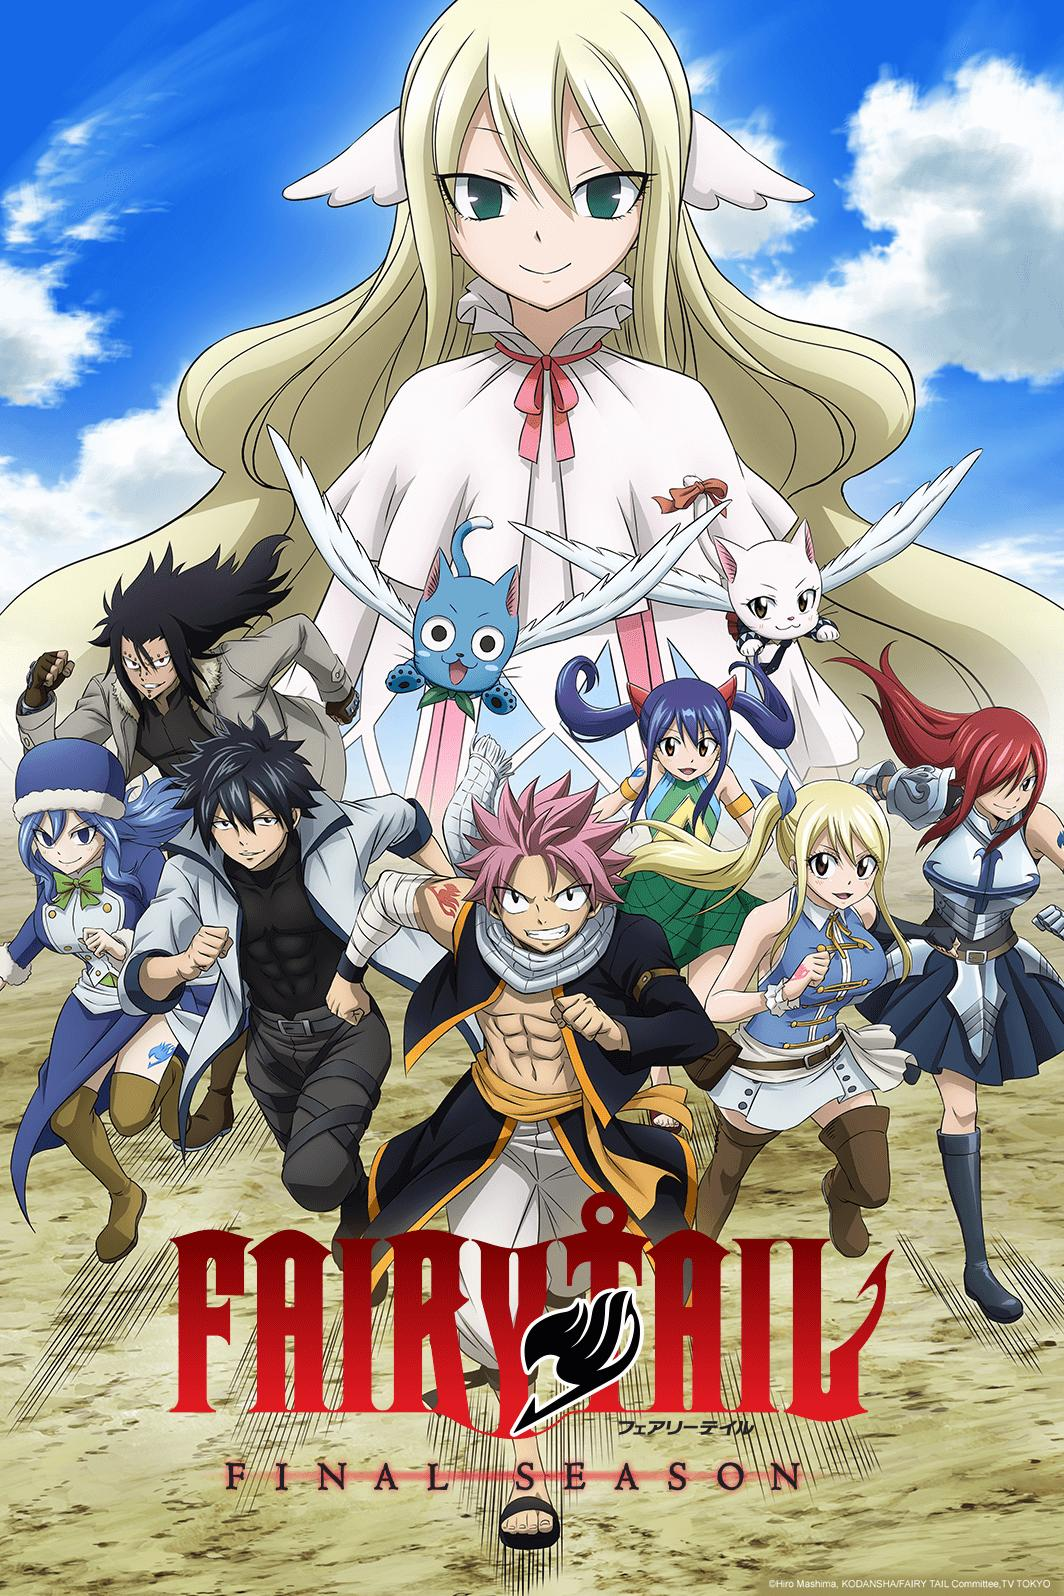
\includegraphics[scale=0.120, angle=15]{Imagenes/Fairy tail.jpg}
      \end{figure}
 %----------------------------------------------------------------------
\section{¿Porque las hadas brillan?}
{\textcolor{Yellow}{Decidí escoger esta serie porque es mi anime favorito}}{\textcolor{orange}{, ya que tiene buenas peleas, buena historia, hay evolución}{\textcolor{red}{en los personajes, igualmente es muy divertido,}}} {\textcolor{Rhodamine}{y principalmente me gusto por que te}}  {\textcolor{Mulberry}{enseña muchos {\huge valores} y por qué te animan a}} {{\textcolor{cyan}{{\huge seguir adelante} y también por que}}} {{\textcolor{ForestGreen}{te mencionan {{\huge frases motivacionales.}}}}}
%-----------------------------------------------------------------------
\begin{SCfigure}[0.999][ht]
     \raggedright
     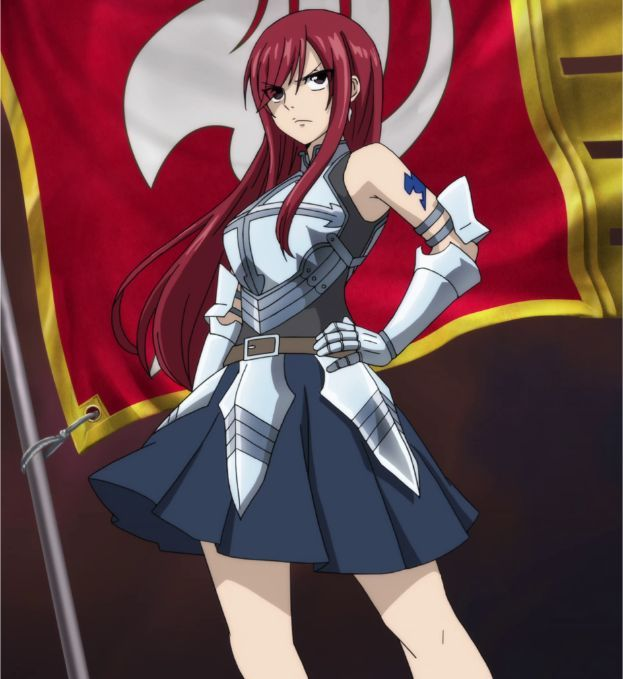
\includegraphics[scale=0.130, angle=-18]{Imagenes/Erza.jpg}
     \caption{\small{{{\textit {Erza Scarlet}}  es mi {\textit{personaje favorito}} y es una maga de clase s y  {\textit {la mas poderosa de fairy Tail}}, viaja con natsu para cumplir con la misiones que aceptan. no obstante tambien realiza misines aparte.}}}
     \label{fig:my_label} 
 \end{SCfigure}
 
\begin{SCfigure}[0.9][ht]
     \raggedright
     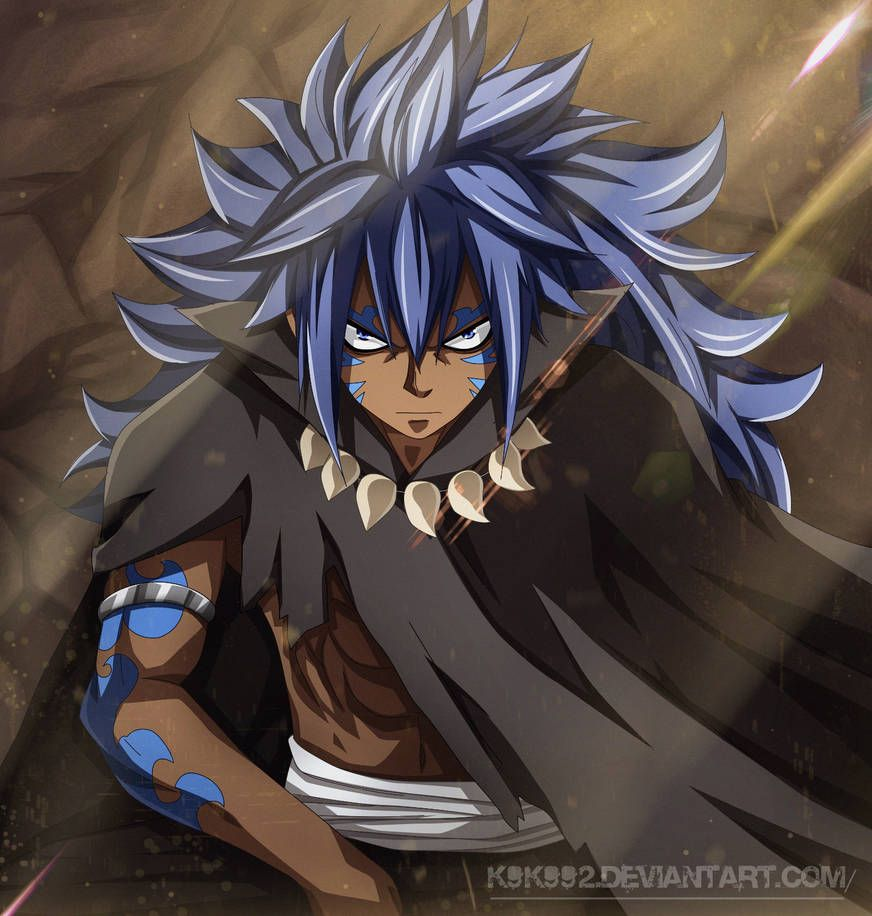
\includegraphics[scale=0.095, angle=8]{Imagenes/Acnologia.jpg}
     \caption{\small{{{\textit {Acnologia}} es mi {\textit {personaje menos favorito}}, es uno de  los {\textit {antagonistas}} principales de la serie, igualmente podemos decir que es uno de los mas {\textit {fuerte}}}}}
     \label{fig:my_label} 
 \end{SCfigure}
%----------------------------------------------------------------------
 \hspace{-3cm}{\textit{\small{``No te des por}}}

\hspace{-3cm}{\textit{\small{vencido, desafía}}}

\hspace{-3cm}{\textit{\small{el presente y cree}}}

\hspace{-3cm}{\textit{\small{en el futuro $\heartsuit$"}}}
\end{document}
